\chapter{Feature Extraction}
\label{ch:feature-extraction}
In this chapter we will talk about feature extraction, which is an essential part of any ML project/workflow.
We will introduce these by looking at a simple example and then look at some more advanced techniques.
After we covered most common approaches we will look into a very important concept, \underline{Machine Learning Pipelines}.

\section{Motivation}
Feature Extraction describes the transformations from any kind of data to vectors.
Until now, we always assumed to have a vector representation of our training data.
We used the notation of $\vec{x} \in \mathbb{R}^d$ to describe a $d$-dimensional data point.
To represent the full data set we used the convention $\vec{X} \in \mathbb{R}^{N \times d}$ 
a $N$-by-$d$ matrix, where each row represents a data point. This notation is commonly used among ML practitioners
and widely implemented in ML libraries. But it is not the only way to represent data. In fact, it is not even the most common way to represent data.
In this chapter we will look into different ways to represent data and how to transform data into a vector representation.

One of the most important things in solving a problem with an ML model is selecting correct features.
Most moder achievements in ML are not due to new algorithms, but due to better ways to extract features.
Thankfully, for most problems we do not need to use any fancy feature extraction techniques or bleeding edge research.
Classical, standard feature extraction techniques are sufficient to solve most problems in a satisfying manner.
In this chapter we will look into some of these techniques, but there are many more.
It is important to underline here, that often the best feature extractors are created by experts with domain knowledge.
Sometimes this expert can be you, but often it is not. In this case it is important to talk to the experts and understand the problem and challenges.
But for many problems and data types there are prebuild methods that we can apply without aquiring the domaing knowledge.
Imagine any work in the Natural Language Processing (NLP) field. It would be horribly bad if every ML practitioner would need to study linguistics prior
to working on an NLP problem.
Lastly, many of theses feature extraction techniques have to be optimized in order to achieve the best results possible. The easiest approach for this is trial and error.

In this chapter we look into four different types of data and different techniques how to extract features from them.

\section{Continuous Features}
Continuous features are the easiest to understand and to work with. They are also the most common type of data.
Continues data, is simply numerical data as real or integer values $x \in \mathbb{R}^d$. In many models continuous features are not required
to be transformed, because they can be used directly. But for some models it is benefitial to normalize continuous features.
For instance if we optimize our model with gradient descent (GD) or when we apply regularization to our model\footnote{Both of these ideas will be introduced in the future, but it is important to mention them here.}.

Given a feature $\vec{x} \in \mathbb{R}^d$ (analog for multivariant) there are several standard normalization options.
\subsection{Normalization: z-Score}
One of the normalization methods foro continuous features is the z-Score or standard scaling.
The z-Score is defined as
\begin{equation}
  z = \frac{x - \mu}{\sigma}
\end{equation}
where $\mu$ is the mean and $\sigma$ is the standard deviation of the feature.

In Python we can implement this as follows:
\begin{lstlisting}[language=Python, caption={z-Score in Python}, label={code:z-score}]
def z_score(X):
  return (X - X.mean(axis=0)) / X.std(axis=0)
\end{lstlisting}
Imagine the data set $\vec{X} \in \mathbb{R}^{N \times 1}$ ($N$ is the number of samples), then we can compute the mean of $\vec{X}$ through \lstinline{X.mean(axis=0)}.
Analogously this approach works for the multivariant case $\vec{X} \in \mathbb{R}^{N \times d}$.
The same applies for the standard deviation \lstinline{X.std(axis=0)}.
Putting everything together we get the z-Score for a data set $\vec{X}$ as implemented in \coderef{code:z-score}.
This method is also implemented in \lstinline{sklearn.preprocessing.StandardScaler}.
\subsection{Normalization: Min-Max-Scaling}
Another form of normalization is Min-Max-Scaling. 
The previous normalization method is great if your data is in the shape of a normal distribution.
If it isn't, you might as well chose Min-Max-Scaling, which ensures that the minimum values $\min(\vec{x})$ and maximum values $\max(\vec{x})$ of the scaled data are in a certain range, e.g. $[0, 1]$.
It does so by computing the min $\min(\vec{x})$ and max $\max(\vec{x})$ of the feature and then scaling the data as follows
\begin{equation}
  x_{scaled} = \frac{x - \min(\vec{x})}{\max(\vec{x}) - \min(\vec{x})}
\end{equation}
The resulting variable is in the range $[0, 1]$ or any other.
This method is also implemented in \lstinline{sklearn.preprocessing.MinMaxScaler}.
The implementation of the Min-Max-Scaling is very similar to the z-Score implementation in \coderef{code:z-score} and can be found in \coderef{code:min-max-scaling}.

\begin{lstlisting}[language=Python, caption={Min-Max-Scaling in Python}, label={code:min-max-scaling}]
def min_max_scaling(X):
  x_min = X.min(axis=0)
  return (
    (X - x_min)
    / (X.max(axis=0) - x_min)
  )
\end{lstlisting}

Similar to the unnormlized data, the normalized data can be used in any ML model.

\section{Categorical Features}
As mentioned earlier continues features often don't need to be trasnformed. But categorical features most certainly need to be transformed.
Categorical features are variables $x \in C$ where $C$ can be any finite set of $N$ values without implicit ordering, e.g.
\begin{itemize}
  \item $C = \{red, green, blue\}$
  \item $C = \{dog, cat, mouse, horse\}$
  \item $C = \{1, 2, 6, 4, 5, 3\}$
  \item $C \in \{\text{User.id}\}$
\end{itemize}
The last example is a bit special, because it is not a finite set. But it is still a categorical feature, because it is not a continues feature.
The first three examples are called \textit{nominal} categorical features, because there is no implicit ordering.
To use these features in a ML model we need to transform them into a vector representation.
Here we will introduce the technique of \textit{One-Hot-Encoding} (OHE) to transform categorical features into a vector representation, but there are also
other techniques like for neural networks so called \textit{Embeddings}.
\subsection{One-Hot-Encoding}
We assume we have a fixed set of categorical values, e.g. $C = \{red, green, blue\}$. Then to generate the one-hot-encoding we first need to compute the cardinality of $C$.
The cardinality of a set is the number of elements in the set. In our example the cardinality of $C$ is $|C| = 3$. This means we need to transform each categorical value into a row-vector of length $|C|$.
For each categorical value we create a vector of length $|C|$ and set the value of the corresponding index to $1$ and all other values to $0$, so that
\begin{itemize}
  \item $red \rightarrow \begin{pmatrix}1 & 0 & 0\end{pmatrix}$
  \item $green \rightarrow \begin{pmatrix}0 & 1 & 0\end{pmatrix}$
  \item $blue \rightarrow \begin{pmatrix}0 & 0 & 1\end{pmatrix}$
\end{itemize}
By doing that categories can be easily represented as vectors.
This is also implemented in \lstinline{sklearn.preprocessing.OneHotEncoder}.
An example for using this approach are bag-of-words vectors, which we will look into in a second.

\subsection{One-hot-Encoding: Problems}
One of the main problems of OHE is that the cardinality of the categorical feature needs to be estimated upfront, i.e. prior to creation of the OHE vectors.
Therefore new items/categories can not be represented. Moreover, we lose the information on similarity between the categories, e.g. "light-blue" is as different as "green" to "blue".

\textbf{Note} In many situations we will face mixtures of continuous and categorical features. Usually we need to apply different extraction methods
to single features to put together a general feature representation of a sample.
\section{Text Features}
The next data type we will look into is text data. Again, we have several options here and especially lately this data type enjoys great popularity and research.
We will look at one approach more closely and shortly touch a few others.
The approach we will focus on is Bag-of-Words (BoW), a simple yet still very powerful technique that is very similar to the one-hot-encoding.
\subsection{Bag-of-Words}
To create BoW-Features we count the word occurrences in the given text. They are basically histograms of word occurrences.

\textbf{Example} Imagine we have the following text
\begin{quote}
  "The tokenizer splits the text into tokens."
\end{quote}
Then we can create a BoW-Feature vector as follows

\begin{table}[h]
  \centering
  \begin{tabular}{|l|ccccccc|}
    \hline
    \textbf{Word} & the & tokenizer & splits & text & into & tokens & . \\
    \hline
    \textbf{Count} & 2 & 1 & 1 & 1 & 1 & 1 & 1 \\
    \hline
  \end{tabular}
  \caption{BoW-Feature vector}
  \label{tab:bow}
\end{table}

How does this work?
\begin{enumerate}
  \item split the text into "tokens", e.g. words
  \item build one-hot-like vector for all found words
  \item count the occurrences of each word inside the text
\end{enumerate}
In the BoW approach $x$ is the vector of word occurrences. The name of an dimension is the word assigned to it.
$\vec{x} \in \mathbb{N}^d$ where $d$ is the number of unique words, the \underline{word vocabulary}, in the text.
$d$ needs to be determined prior to starting and can become quite big, which we will discuss in the following.
\subsubsection{Problems}
BoW-Features only account for the word historgram and due to that most of the natural language structure is lost.
We lose for example the order of words, or context when processing multiple senteces at once.

Overall, BoW-Features are still very efficient and a reasonable approach.

\subsubsection{Model with N-Grams}
To overcome the issue of losing language structure we can apply a different way of tokenizing our text document.
Before we used word-tokens, with N-Grams we use sequences of words, specifically sequences of $N$ words.
E.g. Bi-Grams constst of two words
\begin{table}[h]
  \centering
  \begin{tabular}{|l|ccccc|}
    \hline
    \textbf{Word} & the tokenizer & tokenizer splits & splits the & the text & ...\\
    \hline
    \textbf{Count} & 1 & 1 & 1 & 1 & ... \\
    \hline
  \end{tabular}
  \caption{BoW-Feature Bi-Gram vector}
  \label{tab:bow-bi-gram}
\end{table}
If we would consider every combination of words the dimensionality of this new vector $\vec{x}$ will also significantly change, because we represent sequences of words instead of single words now.
For the Bi-Gram example we get $x \in \mathbb{N}^{d^2}$ where $d$ is the number of unique Bi-Grams in the text.
An implementation of BoW-Features is available in sklearn's \lstinline{sklearn.feature_extraction.text.CountVectorizer}.

\subsubsection{Character N-Grams}
We will briefly look into another approach to BoW-Features, which is using character N-Grams instead of word N-Grams.
This approach uses character sequences instead of word sequences. This approach is especially useful for languages with a rich morphology, e.g. German.
Another great application is for language independent models, e.g. for language detection.
Eseentially, we can select a tokenization method that fits our needs best, then transform these tokens into a BoW encoding.

\subsubsection{Term Frequency - Inverse Document Frequency (TF-IDF)}
One of the problems of using token occurrences is that natural language contains a lot of words that don't transfer information.
Frequently occurring words like "the" are often not meaningful and will be weighted down by the inverse document frequency.
Usually, we see a word-frequency distribution in the shape of the distribution shown in Figure \ref{fig:word-freq-dist}.

\begin{figure}[h]
  \centering
  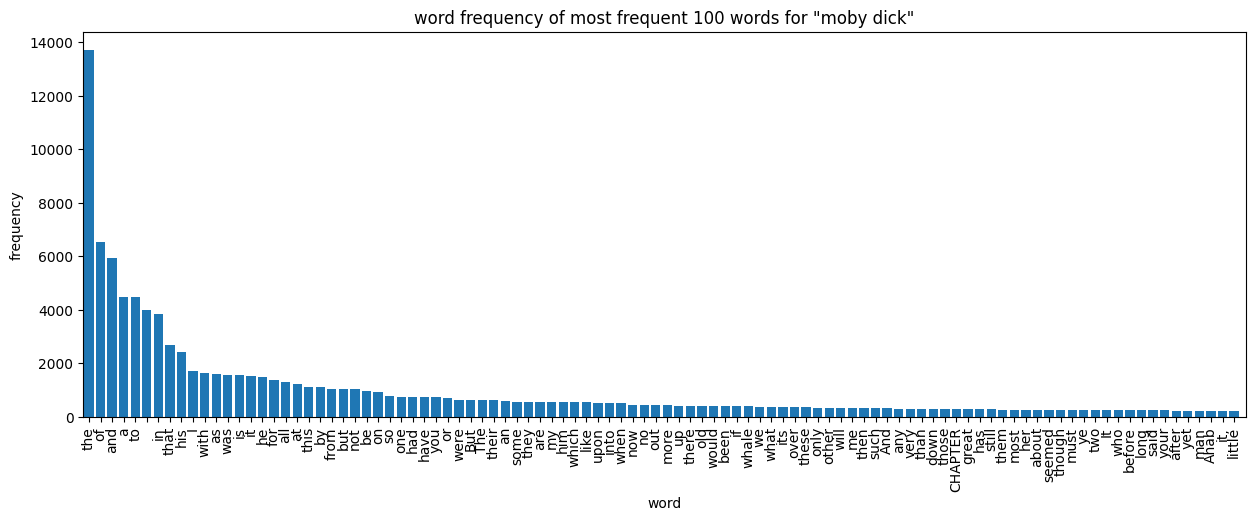
\includegraphics[width=.95\textwidth]{images/word-distribution.png}
  \caption{Word frequency distribution of 100 most frequent words in Moby Dick (https://www.gutenberg.org/ebooks/2701)}
  \label{fig:word-freq-dist}
\end{figure}
In order to downweight the frequently occurring words, to be able to only select relevant words, we apply the inverse
document frequency
\begin{equation}
  \text{idf}(t, d) = \log \frac{|d|}{|d \text{ containing } t|}
  \label{eq:IDF}
\end{equation}
This document frequency can be combined with the term frequency, the number of occurrences of a single word/token $|t|$ over the number of occurring words/tokens $|d|$
\begin{equation}
  \text{tf}(t, d) = \frac{|t|}{|d|}
  \label{eq:TF}
\end{equation}
tf \eqref{eq:TF} and idf \eqref{eq:IDF} can be combined by forming their product
\begin{equation}
  \text{tfidf}(t, d) = \text{tf}(t, d) \cdot \text{idf}(t, d)
  \label{eq:TF-IDF}
\end{equation}
A model incorporating this metric is TFIDF which is essentially a BoW model with applied term frequency and idf.

In sklearn you can find it under \lstinline{sklearn.feature_extraction.text.TfidfVectorizer}.

\subsubsection{Stop-Words}
Another alternative to remove noice from our data are Stop-Words.
Instead of computing tf and idf, we have a set of predefined words to exclude from the document.
For most languages we can do that and prepare a set of words that won't change frequently.
From my experience they seem to work great, and I use them more often than TF-IDF.

\subsubsection{Expensive N-Grams}
We quickly jump back to the N-Gram tokens and discuss the dimensionality of our BoW vectors.

If we use unigrams ($N = 1$) the size of our vectors $\vec{x} \in \mathbb{R}^d$ is $d$ the size of our vocabulary.
The size of this is $v$ in the worst case. Libraries use so called sparse vectors to represent these
high dimensional data points, dense representations require too much memory by storing $0$ values.
When we increase $N$ to $N=2$ (Bi-Grams) this memory requirement grows by a factor of $d$. So the worst case
scenario increases to $d^2 \Rightarrow \vec{x} \in \mathbb{R}^{d^2}$.
But mostly we do not gain much from this, in terms of increasing the context that is encoded.
This applies annalogously to higher orders of N-Grams, e.g. $N=3$ (Tri-Grams) require $V^3$ dimensions and so on.
If we consider e.g. German as a language, and we know that the vocabulary for this language is somewhere in the realm of $d \approx 10^{12}$.
This will cause big memory issues, especially when using anything else but Uni-Grams.

Before neural networks and deep learning google provided big sets of N-Gram data for many languages, so no one must create them
themself. You can find up to $N=5$-Grams here: \url{http://storage.googleapis.com/books/ngrams/books/datasetsv2.html}.

\subsubsection{Hashed N-Grams}
Another optimization trick to reduce memory of N-Grams is using hash-maps.

For those who know about hash-maps, instead of representing words/tokens as vectors, each dimension corresponds to a hash bucket
using a hash function.
This can cause hash-collision, a problem where two or more values are hashed to the same hash-value. It appears when the number of hash-buckets
is lower than the number of $N$-Grams we want to store.
But because of the structure of natural language we rarely have multiple senteces containing the same words in different orders, the collision rate is low to insignificant.
I highly encourage the reader to try it out, if you run out of memory with regular vectorizers.

For those of you who don't know about hash-maps, you can think of it as a dictionary, where each word is a key and the value is the number of occurrences, you can read more about
the inner workings of hash maps in the great 2020 blog post by Adam Gold \cite{adamgold:hash-maps}.

\subsubsection{Example \#1}
Let us look at an example of how to use these techniques in Python on a specific task.
We will use the 20 newsgroups data set, which is a collection of 20,000 newsgroup documents, partitioned (nearly) evenly across all newsgroups.
You can find more information about this data set here: \url{http://qwone.com/~jason/20Newsgroups/}.
Essentially, we will train a model to classify the newsgroup of a given document.
We will use the \lstinline{sklearn.datasets.fetch_20newsgroups} function to download the data set and then use the \lstinline{sklearn.feature_extraction.text.TfidfVectorizer}
to transform the text into a BoW representation.
After that we will train a NCC model and KNN model on the data set.
\begin{lstlisting}[language=Python, caption={20 newsgroups example}, label={code:20-newsgroups}]
from sklearn.datasets import fetch_20newsgroups
from sklearn.feature_extraction.text import TfidfVectorizer
from sklearn.neighbors import NearestCentroid, KNeighborsClassifier

# Download the data set
newsgroups_train = fetch_20newsgroups(subset='train')
newsgroups_test = fetch_20newsgroups(subset='test')

# Transform the text into a BoW representation
vectorizer = TfidfVectorizer()
X_train = vectorizer.fit_transform(newsgroups_train.data)
X_test = vectorizer.transform(newsgroups_test.data)

# Train a Nearest Centroid Classifier
clf = NearestCentroid()
clf.fit(X_train, newsgroups_train.target)
acc = (clf.predict(X_test) == imdb_test.target).mean()
print(f"Accuracy: {acc}")

# Train a KNN Classifier
clf = KNeighborsClassifier()
clf.fit(X_train, newsgroups_train.target)
acc = (clf.predict(X_test) == imdb_test.target).mean()
print(f"Accuracy: {acc}")
\end{lstlisting}

\begin{table}[h]
  \centering
  \begin{tabular}{|l|c|}
    \hline
    \textbf{Model} & \textbf{Accuracy} \\
    \hline
    \textbf{Nearest Centroid Classifier} & \textbf{0.692113648433351}\\
    K-Nearest Neighbors Classifier & 0.6591874668082847\\
    \hline
  \end{tabular}
  \caption{Accuracy of NCC and KNN on 20 newsgroups data set}
  \label{tab:20-newsgroups}
\end{table}

Running the code in \coderef{code:20-newsgroups} will result in the accuracy scores shown in Table \ref{tab:20-newsgroups}.
You will notice that albeit the simplicity of the NCC model it performs better than the KNN model. Furthermore, the NCC model is also substantially faster to train.

A better approach for this problem would be to use the Logistic Regression (LogReg) model. We will look into this model in the future (Chapter \ref{ch:regression}), for now we will consider it a black box and apply it to the news group data set to demonstrate its performance on this task.

\begin{lstlisting}[language=Python, caption={20 newsgroups example with Logistic Regression}, label={code:20-newsgroups-lr}]
from sklearn.datasets import fetch_20newsgroups
from sklearn.feature_extraction.text import TfidfVectorizer
from sklearn.linear_model import LogisticRegression

# Download the data set
newsgroups_train = fetch_20newsgroups(subset='train')
newsgroups_test = fetch_20newsgroups(subset='test')

# Transform the text into a BoW representation
vectorizer = TfidfVectorizer()
X_train = vectorizer.fit_transform(newsgroups_train.data)
X_test = vectorizer.transform(newsgroups_test.data)

# Train a Logistic Regression Classifier
clf = LogisticRegression(random_state=0)
clf.fit(X_train, newsgroups_train.target)
print(f"Accuracy: {clf.score(X_test, newsgroups_test.target)}")
\end{lstlisting}
\begin{table}[h]
  \centering
  \begin{tabular}{|l|c|}
    \hline
    \textbf{Model} & \textbf{Accuracy} \\
    \hline
    Nearest Centroid Classifier & 0.692113648433351\\
    K-Nearest Neighbors Classifier & 0.6591874668082847\\
    \textbf{LogisticRegression} & \textbf{0.8274030801911842}\\
    \hline
  \end{tabular}
  \caption{Accuracy of NCC, KNN and LogReg on 20 newsgroups data set}
  \label{tab:20-newsgroups-extended}
\end{table}
After running the code in \coderef{code:20-newsgroups-lr} we can see that the LogReg model performs significantly better than the NCC and KNN models (see Table \ref{tab:20-newsgroups-extended}).
This is due to the fact that the LogReg model is able to learn non-linear decision boundaries, which the NCC and KNN models are not able to do, because they are linear classifiers.
We will look into LogReg in the future, but for now it is important to understand that the NCC model is a linear classifier and therefore can only learn linear decision boundaries.
And apparently, the data set is not linearly separable, which is why the linear classification models perform so poorly.

\subsubsection{Example \#2}
In this example we will look into a different data set, the \textit{IMDB} data set~\cite{maas-EtAl:2011:ACL-HLT2011} (\url{http://ai.stanford.edu/~amaas/data/sentiment/}).
This data set contains 50,000 movie reviews from the Internet Movie Database, labeled by sentiment (positive/negative/unsupervised).
We will use the \lstinline{sklearn.datasets.load_files} function to download the data set and then use the \lstinline{sklearn.feature_extraction.text.TfidfVectorizer}
to transform the text into a BoW representation.
Similar to the previous example, we will classify the reviews using a NCC model and a LinReg model.

\begin{lstlisting}[language=Python, caption={IMDB example}, label={code:imdb}]
from sklearn.datasets import load_files
from sklearn.feature_extraction.text import TfidfVectorizer
from sklearn.neighbors import NearestCentroid
from sklearn.linear_model import LogisticRegression

# load the data set
imdb_train = load_files('aclImdb/train')
imdb_test = load_files('aclImdb/test')

# Transform the text into a BoW representation
vectorizer = TfidfVectorizer()
X_train = vectorizer.fit_transform(imdb_train.data)
X_test = vectorizer.transform(imdb_test.data)

# Train a Nearest Centroid Classifier
clf = NearestCentroid()
clf.fit(X_train, imdb_train.target)
print(f"Accuracy: {clf.score(X_test, imdb_test.target)}")

# Train a Logistic Regression Classifier
clf = LogisticRegression(random_state=42, solver='newton-cg', C=100.)
clf.fit(X_train, imdb_train.target)
acc = (clf.predict(X_test) == imdb_test.target).mean()
print(f"Accuracy: {acc}")
\end{lstlisting}
As the results in Table \ref{tab:imdb} show, the NCC model performs better on this task than the LogReg model.
\begin{table}[h]
  \centering
  \begin{tabular}{|l|c|}
    \hline
    \textbf{Model} & \textbf{Accuracy} \\
    \hline
    \textbf{Nearest Centroid Classifier} & \textbf{0.62312}\\
    Logistic Regression & 0.19984\\
    \hline
  \end{tabular}
  \caption{Accuracy of NCC and LogReg on IMDB data set}
  \label{tab:imdb}
\end{table}
But an accuracy of 62.31\% is not very good, especially considering that a random guess would result in an accuracy of 33.3\%.
One option would be to reduce the problem to a binary classification problem, i.e. positive or negative sentiment.
Doing so would result in an accuracy of 62.89\% for the NCC model and 17.56\% for the LogReg model.
As you can see, the NCC model still performs better than the LogReg model, but still not very good, frankly the improvement was rather sobering.

To improve on the $\approx 60\%$ accuracy we could use a different model architecture, e.g. a neural network.
In future chapters we will look closer into the architecture powering so called Multi-Layer Perceptrons (MLPs).
But for now it is important to understand that MLPs are able to learn non-linear decision boundaries, which is why they are able to perform better on this task.

Implementing an MLP is as easy as replacing the NCC model with a MLP model from the \lstinline{sklearn.neural_network.MLPClassifier} class.
\begin{lstlisting}[language=Python, caption={IMDB example with MLP}, label={code:imdb-mlp}]
from sklearn.datasets import load_files
from sklearn.feature_extraction.text import TfidfVectorizer
from sklearn.neural_network import MLPClassifier

# load the data set
imdb_train = load_files('aclImdb/train')
imdb_test = load_files('aclImdb/test')

# Transform the text into a BoW representation
vectorizer = TfidfVectorizer()
X_train = vectorizer.fit_transform(imdb_train.data)
X_test = vectorizer.transform(imdb_test.data)

# Train a MLP Classifier
clf = MLPClassifier(
  hidden_layer_sizes=(100, 100),
  max_iter=10,
  alpha=1e-4,
  solver='sgd',
  verbose=10,
  random_state=42,
  learning_rate_init=.1
)
clf.fit(X_train, imdb_train.target)
acc = (clf.predict(X_test) == imdb_test.target).mean()
print(f"Accuracy: {acc}")
\end{lstlisting}
The results in Table \ref{tab:imdb-mlp} show that the MLP model performs significantly better than the NCC and LogReg models.

\begin{table}[h]
  \centering
  \begin{tabular}{|l|c|}
    \hline
    \textbf{Model} & \textbf{Accuracy} \\
    \hline
    Nearest Centroid Classifier & 0.62312\\
    Logistic Regression & 0.19984\\
    \textbf{MLP Classifier} & \textbf{0.849}\\
    \hline
  \end{tabular}
  \caption{Accuracy of NCC, LogReg and MLP on IMDB data set}
  \label{tab:imdb-mlp}
\end{table}
Great, we were able to improve the accuracy from $\approx 60\%$ to $\approx 85\%$.

But this can't be it. We can do better than that. And we will.

A more advanced technique is to use word embeddings, which we will look into now.
\subsection{Word Embeddings}
The following section describes techniques which apply neural networks to generate word embeddings.
For now, we will look into how to use these embeddings as feature extractors.
Later, in Chapters \ref{ch:neural-networks} and \ref{ch:deep-learning}, we will look into how to train these embeddings models and how to use them for other tasks.
Word embeddings are a more advanced technique to represent words as vectors as the previosuly introduced OHE approach of BoW.\\
Over the past two years word embeddings have enjoyed great popularity and research among the ML community.
Especially with the rise of Large Language Models (LLMs) like BERT\cite{devlin2019bert} and GPT-3\cite{brown2020language}, the introduction of ChatGPT\cite{ChatGPT:2022} in late 2022 and the groundbreaking Open Source community around architectures of 2023 like LLaMa\cite{touvron2023llama}, LLaMa2\cite{touvron2023llama2} and Mixtral\cite{mixtral:2023}, these vectors became more and more relevant.

They are a dense representation of words, which means that they do not contain many $0$ values.
This is in contrast to the sparse representation of BoW-Features, which contain many $0$ values.
Word embeddings are usually trained on a large corpus of text, e.g. Wikipedia, and then used as a feature extractor for other tasks.
The most popular word embedding is the \textit{Word2Vec} embedding, which is trained on a large corpus of text coming from Wikipedia.
Word Embeddings are quite versatile, they can be used for many different tasks, e.g. word similarity, word analogies, text classification, etc.
We will look into the word similarity and word analogy tasks in a future chapter.
The quintessence of Word Embeddings is that they are able to encode semantic and syntactic information of words.
The most prominent example to demonstrate this encoded information is the following.

Let the embedding vector for the word "King" be $\vec{a} = \begin{pmatrix}1 & 1 & 0\end{pmatrix}$, the embedding vector of the word "Man" $\vec{b} = \begin{pmatrix}1 & 0 & 0\end{pmatrix}$ and the embedding vector for the word "Woman" be $\vec{c} = \begin{pmatrix}0 & 0 & 1\end{pmatrix}$.
  Then we can compute the embedding vector for the word "Queen" $\vec{d}$ by subtracting "Man" from "King" and adding "Woman" to create $\vec{d} = a - b + c = \begin{pmatrix}0 & 1 & 1\end{pmatrix}$.

This is of course a great simplification of the actual process. Embedding vectors have way more than just 3 dimensions and will most likely not contain beautiful integers as in this example.

We will look in Chapter \ref{ch:pca} into a technique called Principal Component Analysis (PCA), which can be used to reduce the dimensionality of embedding vectors to 2 or 3 dimensions. 
This allows us to visualize these high dimensional vectors.

You can check out \url{https://projector.tensorflow.org/} for a great visualization of word embeddings.

\subsubsection{Word2Vec}
Word2Vec is a word embedding technique that was introduced in 2013 by Mikolov et al. \cite{mikolov2013efficient}.
The idea behind Word2Vec is to train a neural network to predict the context of a word.
The context of a word is defined as the words surrounding the word in a given text.
The neural network is trained on a large corpus of text, e.g. Wikipedia, and then used as a feature extractor for other tasks.
A library that implements Word2Vec is \lstinline{gensim} \\(\url{https://radimrehurek.com/gensim/}).
Using Word2Vec is as easy as downloading a pre-trained model and then using it as a feature extractor.
\begin{lstlisting}[language=Python, caption={Word2Vec example}, label={code:word2vec}]
import gensim.downloader as api

# Download the pre-trained model
model = api.load("word2vec-google-news-300")

# Get the embedding vector for the word "King"
print(model["king"])
\end{lstlisting}
The code in \coderef{code:word2vec} will download the pre-trained Word2Vec model ($\approx$1.7 GB) from Google and then print the embedding vector for the word "King".

As you can see, we can generate embeddings for single words, but also for sentences and even paragraphs.Albeit the flexibility of the Word2Vec model, the model is not capable of generating embeddings for unknown words, i.e. words that are not in the original training vocabulary, e.g. "Kinging" and "Queening". 
This is a problem that is solved by the FastText model, which we will look into in the next section.

\subsubsection{FastText}
FastText is a word embedding technique that was introduced in 2016 by Bojanowski et al. \cite{bojanowski2016enriching}.
The idea behind FastText is to train a neural network to predict the context of a word, similar to Word2Vec.
But instead of using words as the smallest unit, FastText uses character N-Grams.
This allows FastText to generate embeddings for unknown words, i.e. words that are not in the original training vocabulary, e.g. "Kinging" and "Queening".
Gensim also provides a FastText model, which can be used in the same way as the Word2Vec model.
\begin{lstlisting}[language=Python, caption={FastText example}, label={code:fasttext}]
import gensim.downloader as api

# Download the pre-trained model
model = api.load("fasttext-wiki-news-subwords-300")

# Get the embedding vector for the word "King"
print(model["king"])
\end{lstlisting}
The code in \coderef{code:fasttext} will download the pre-trained FastText model ($\approx$1 GB) from Wikipedia and then print the embedding vector for the word "King".

\subsubsection{GloVe}
Another word embedding technique is GloVe, which was introduced in 2014 by Pennington et al. \cite{pennington2014glove}.
Other than FastText and Word2Vec, GloVe is not a neural network based model, but a matrix factorization technique.
The idea behind GloVe is to factorize the word-word co-occurrence matrix.
The word-word co-occurrence matrix is a matrix that contains the number of times a word $i$ appears in the context of word $j$.
The GloVe model is also available in Gensim.
\begin{lstlisting}[language=Python, caption={GloVe example}, label={code:glove}]
import gensim.downloader as api

# Download the pre-trained model
model = api.load("glove-wiki-gigaword-300")

# Get the embedding vector for the word "King"
print(model["king"])
\end{lstlisting}
The code in \coderef{code:glove} will download the pre-trained GloVe model ($\approx$1.4 GB) from Wikipedia and then print the embedding vector for the word "King".

\subsubsection{Comparison}
Now that we have looked into three different word embedding techniques, let us compare them.
We will use the same example as in the previous section, the 20 newsgroups data set.
We will use the \lstinline{sklearn.datasets.fetch_20newsgroups} function to download the data set and then use the embedding models to transform the text into a vector representation.
After that we will train a NCC model and MLP model on the data set.

\framedtext{\color{red}{TODO:} Code sample not working, fix it}

\begin{lstlisting}[language=Python, caption={20 newsgroups example with embeddings}, label={code:20-newsgroups-embeddings}]
from sklearn.datasets import fetch_20newsgroups
from sklearn.neighbors import NearestCentroid
from sklearn.neural_network import MLPClassifier
import gensim.downloader as api

# Download the data set
newsgroups_train = fetch_20newsgroups(subset='train')
newsgroups_test = fetch_20newsgroups(subset='test')

# Download the pre-trained models
word2vec_model = api.load("word2vec-google-news-300")
fasttext_model = api.load("fasttext-wiki-news-subwords-300")
glove_model = api.load("glove-wiki-gigaword-300")

# Transform the text into a vector representation
X_train_word2vec = [word2vec_model[x] for x in newsgroups_train.data]
X_test_word2vec = [word2vec_model[x] for x in newsgroups_test.data]
# Train a Nearest Centroid Classifier
clf = NearestCentroid()
clf.fit(X_train_word2vec, newsgroups_train.target)

# Train a MLP classifier
clf = MLPClassifier(
  max_iter=10,
  verbose=10,
  random_state=42,
)
clf.fit(X_train_word2vec, newsgroups_train.target)

print("Word2Vec")
print(f"NCC Accuracy: {clf.score(X_test_word2vec, newsgroups_test.target)}")
print(f"MLP Accuracy: {(clf.predict(X_test_word2vec) == newsgroups_test.target).mean()}")

del X_train_word2vec, X_test_word2vec

X_train_fasttext = [fasttext_model[x] for x in newsgroups_train.data]
X_test_fasttext = [fasttext_model[x] for x in newsgroups_test.data]

# Train a Nearest Centroid Classifier
clf = NearestCentroid()
clf.fit(X_train_fasttext, newsgroups_train.target)

# Train a MLP classifier
clf = MLPClassifier(
  max_iter=10,
  verbose=10,
  random_state=42,
)
clf.fit(X_train_fasttext, newsgroups_train.target)

print("FastText")
print(f"NCC Accuracy: {clf.score(X_test_fasttext, newsgroups_test.target)}")
print(f"MLP Accuracy: {(clf.predict(X_test_fasttext) == newsgroups_test.target).mean()}")
del X_train_fasttext, X_test_fasttext

X_train_glove = [glove_model[x] for x in newsgroups_train.data]
X_test_glove = [glove_model[x] for x in newsgroups_test.data]

# Train a Nearest Centroid Classifier
clf = NearestCentroid()
clf.fit(X_train_glove, newsgroups_train.target)

# Train a MLP Classifier
clf = MLPClassifier(
  max_iter=10,
  verbose=10,
  random_state=42,
)
clf.fit(X_train_glove, newsgroups_train.target)

print("GloVe")
print(f"NCC Accuracy: {clf.score(X_test_glove, newsgroups_test.target)}")
print(f"MLP Accuracy: {(clf.predict(X_test_glove) == newsgroups_test.target).mean()}")
\end{lstlisting}
The code in \coderef{code:20-newsgroups-embeddings} will download the pre-trained embedding models and then transform the text into a vector representation.
After that we train a NCC model and MLP model on the data set.

\section{Image Features}
We discussed until now continuous and categorical features, as well as text features.
To complete this we will briefly look at methods to extract features from images.
Due to the complexity of these methods we will only motivate them, because thoroughly understanding them would go beyond the scope of this book.
Most of them are very easy to use, but hard to understand.

\subsection{Classic Computer Vision}
Before 2012 (ImageNet Moment) researches used classic CV methods to extract features from images.
Mostly Furrier Decomposition was applied, this measures spacial frequencies of patches of the image.
The resulting frequency strength of each patch is then used as a feature.
These spacial frequencies are gradients in the image. High spacial frequencies are edges,
and the phase of the frequency is its orientation.
These kind of features are computed in the \underline{Histogram of Oriented Gradients/Edges} (HOG) feature extractor, as showcased in 
Figure \ref{fig:hog}.

\begin{figure}[h]
  \centering
  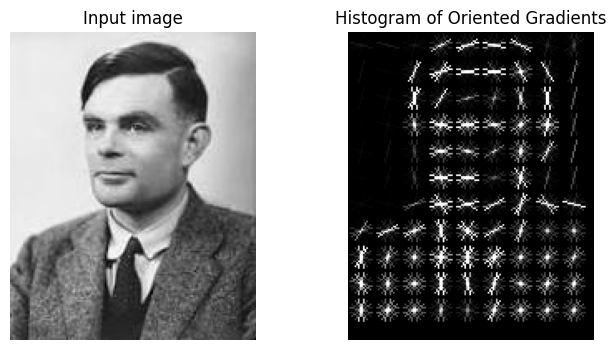
\includegraphics[width=.95\textwidth]{images/hog.png}
  \caption{HOG feature extraction}
  \label{fig:hog}
\end{figure}

HOG suits very well for object detection, because it is very robust to changes in illumination and other factors.
For this reason it is widely used in e.g. self-driving cars for pedestrian recognition.
They work good if we only want to encode a shape, e.g. a pedestrian, but not for more complex tasks like face recognition.
In skimage you can find the HOG extractor in \lstinline{skimage.feature.hog}.

\subsection{Convolutional Neural Networks}
Another more modern way of dealing with images is using Convolutional Neural Networks (CNNs).
They are state-of-the-art (SOTA) for image classification and object detection.
We don't have much time to look detaied into them, but the key takeaway here is:

We won't train these models from scratch. We will apply pretrained models, because we won't
be able to achieve same performance with models we would train ourselves.
And we don't want to spend so much time and money on training these models.
Thankfully, we don't need to because there are many pretrained models publicly available.
These models are trained foro a long time on very large datasets, e.g. ImageNet\cite{deng2009imagenet}, for us!
All we have to do is to download these models and run them as feature extractors.
You can read more about CNNs in \cite{PhilippZettl:2022} or Chapter \ref{ch:neural-networks}.


Essentially, CNNs are combinations of convolutional filter masks that are stacked on top of each other adding more and more complexity to the model.
The first layers learn simple features like edges and the last layers learn more complex features like shapes and objects.
The last layers are then used as features for our ML model.
Originally, when using the ImageNet data set, the models are trained on the image classification task.
But we can use the features of the last layers for any other task, e.g. object detection, because the features are still very meaningful and valid.
Instead of using the full pretrained model, we can also use only the first layers of the model and train the last layers on our own data set, or we simply
only use the first few pretrained layers as feature extractors.

You can see the representation of different channels from a specific layer in Figure \ref{fig:cnn-features} as well as the combination of all channels in Figure \ref{fig:cnn-features-1}.

\begin{figure}[h]
  \centering
  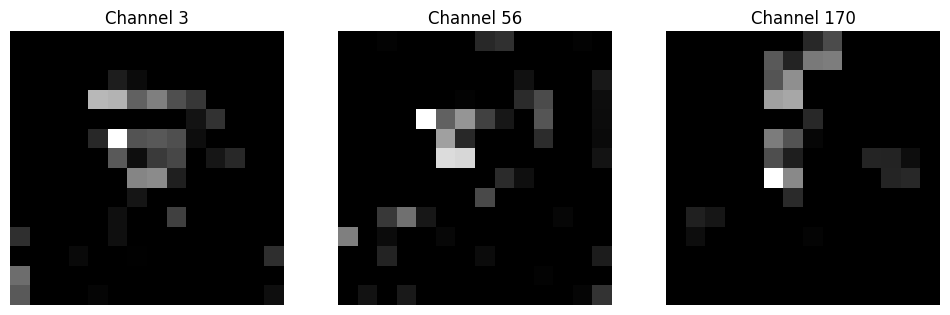
\includegraphics[width=.95\textwidth]{images/cnn-0.png}
  \caption{CNN feature extraction of different channels}
  \label{fig:cnn-features}
\end{figure}

\begin{figure}[h]
  \centering
  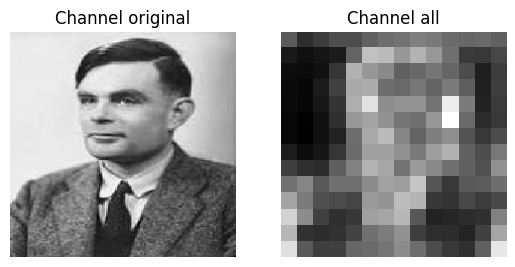
\includegraphics[width=.95\textwidth]{images/cnn-1.png}
  \caption{CNN feature channels combined}
  \label{fig:cnn-features-1}
\end{figure}

You can imagine image channels as a encoding of spacial frequencies, similar to the HOG features.
But other than HOG features, CNNs are able to learn these features in a general way by themselves, which is why they are so powerful.

Consider this, color images have three channels, red, green and blue. Each of these channels encodes a different spacial frequency.
Let $X \in \mathbb{R}^{H \times W \times 3}$ be an image with height $H$, width $W$ and three channels and random content (see Figure \ref{fig:channels}).
Then we can define three matrices $T_{red}, T_{green}, T_{blue} \in \mathbb{R}^{H \times W \times 3}$ that select the corresponding channel of each pixel.
\begin{align}
  \begin{pmatrix}
    \{\vec{x}_{1,1,1},\vec{x}_{1,1,2},\vec{x}_{1,1,3}\}
    & \{\vec{x}_{1,2,1},\vec{x}_{1,2,2},\vec{x}_{1,2,3}\}
    & \dots
    & \{\vec{x}_{1,W,1},\vec{x}_{1,W,2},\vec{x}_{1,W,3}\} \\
    \{\vec{x}_{2,1,1},\vec{x}_{2,1,2},\vec{x}_{2,1,3}\}
    & \{\vec{x}_{2,2,1},\vec{x}_{2,2,2},\vec{x}_{2,2,3}\}
    & \dots
    & \{\vec{x}_{2,W,1},\vec{x}_{2,W,2},\vec{x}_{2,W,3}\} \\
    \vdots & \vdots & \ddots & \vdots \\
    \{\vec{x}_{H,1,1},\vec{x}_{H,1,2},\vec{x}_{H,1,3}\}
    & \{\vec{x}_{H,2,1},\vec{x}_{H,2,2},\vec{x}_{H,2,3}\}
    & \dots
    & \{\vec{x}_{H,W,1},\vec{x}_{H,W,2},\vec{x}_{H,W,3}\}
  \end{pmatrix}
\end{align}
Then we can extract the three channels as follows.
For the red channel we select the first channel of each pixel
\begin{align}
  T_{red} = \begin{pmatrix}
    \{1, 0, 0\}
    & \{1, 0, 0\}
    & \dots
    & \{1, 0, 0\}\\
    \{1, 0, 0\}
    & \{1, 0, 0\}
    & \dots
    & \{1, 0, 0\}\\
    \vdots & \vdots & \ddots & \vdots \\
    \{1, 0, 0\}
    & \{1, 0, 0\}
    & \dots
    & \{1, 0, 0\}
  \end{pmatrix}
\end{align}
For the green channel we select the second channel of each pixel
\begin{align}
  T_{green} = \begin{pmatrix}
    \{0, 1, 0\}
    & \{0, 1, 0\}
    & \dots
    & \{0, 1, 0\}\\
    \{0, 1, 0\}
    & \{0, 1, 0\}
    & \dots
    & \{0, 1, 0\}\\
    \vdots & \vdots & \ddots & \vdots \\
    \{0, 1, 0\}
    & \{0, 1, 0\}
    & \dots
    & \{0, 1, 0\}
  \end{pmatrix}
\end{align}
And for the blue channel we select the third channel of each pixel
\begin{align}
  T_{blue} = \begin{pmatrix}
    \{0, 0, 1\}
    & \{0, 0, 1\}
    & \dots
    & \{0, 0, 1\}\\
    \{0, 0, 1\}
    & \{0, 0, 1\}
    & \dots
    & \{0, 0, 1\}\\
    \vdots & \vdots & \ddots & \vdots \\
    \{0, 0, 1\}
    & \{0, 0, 1\}
    & \dots
    & \{0, 0, 1\}
  \end{pmatrix}
\end{align}

Applying those three matrices to our image $X$ we get three images $X_{red}, X_{green}, X_{blue} \in \mathbb{R}^{H \times W \times 3}$ as individually shown in Figure \ref{fig:channels-individual}.
\begin{figure}
  \centering
\begin{minipage}[t]{.3\textwidth}
  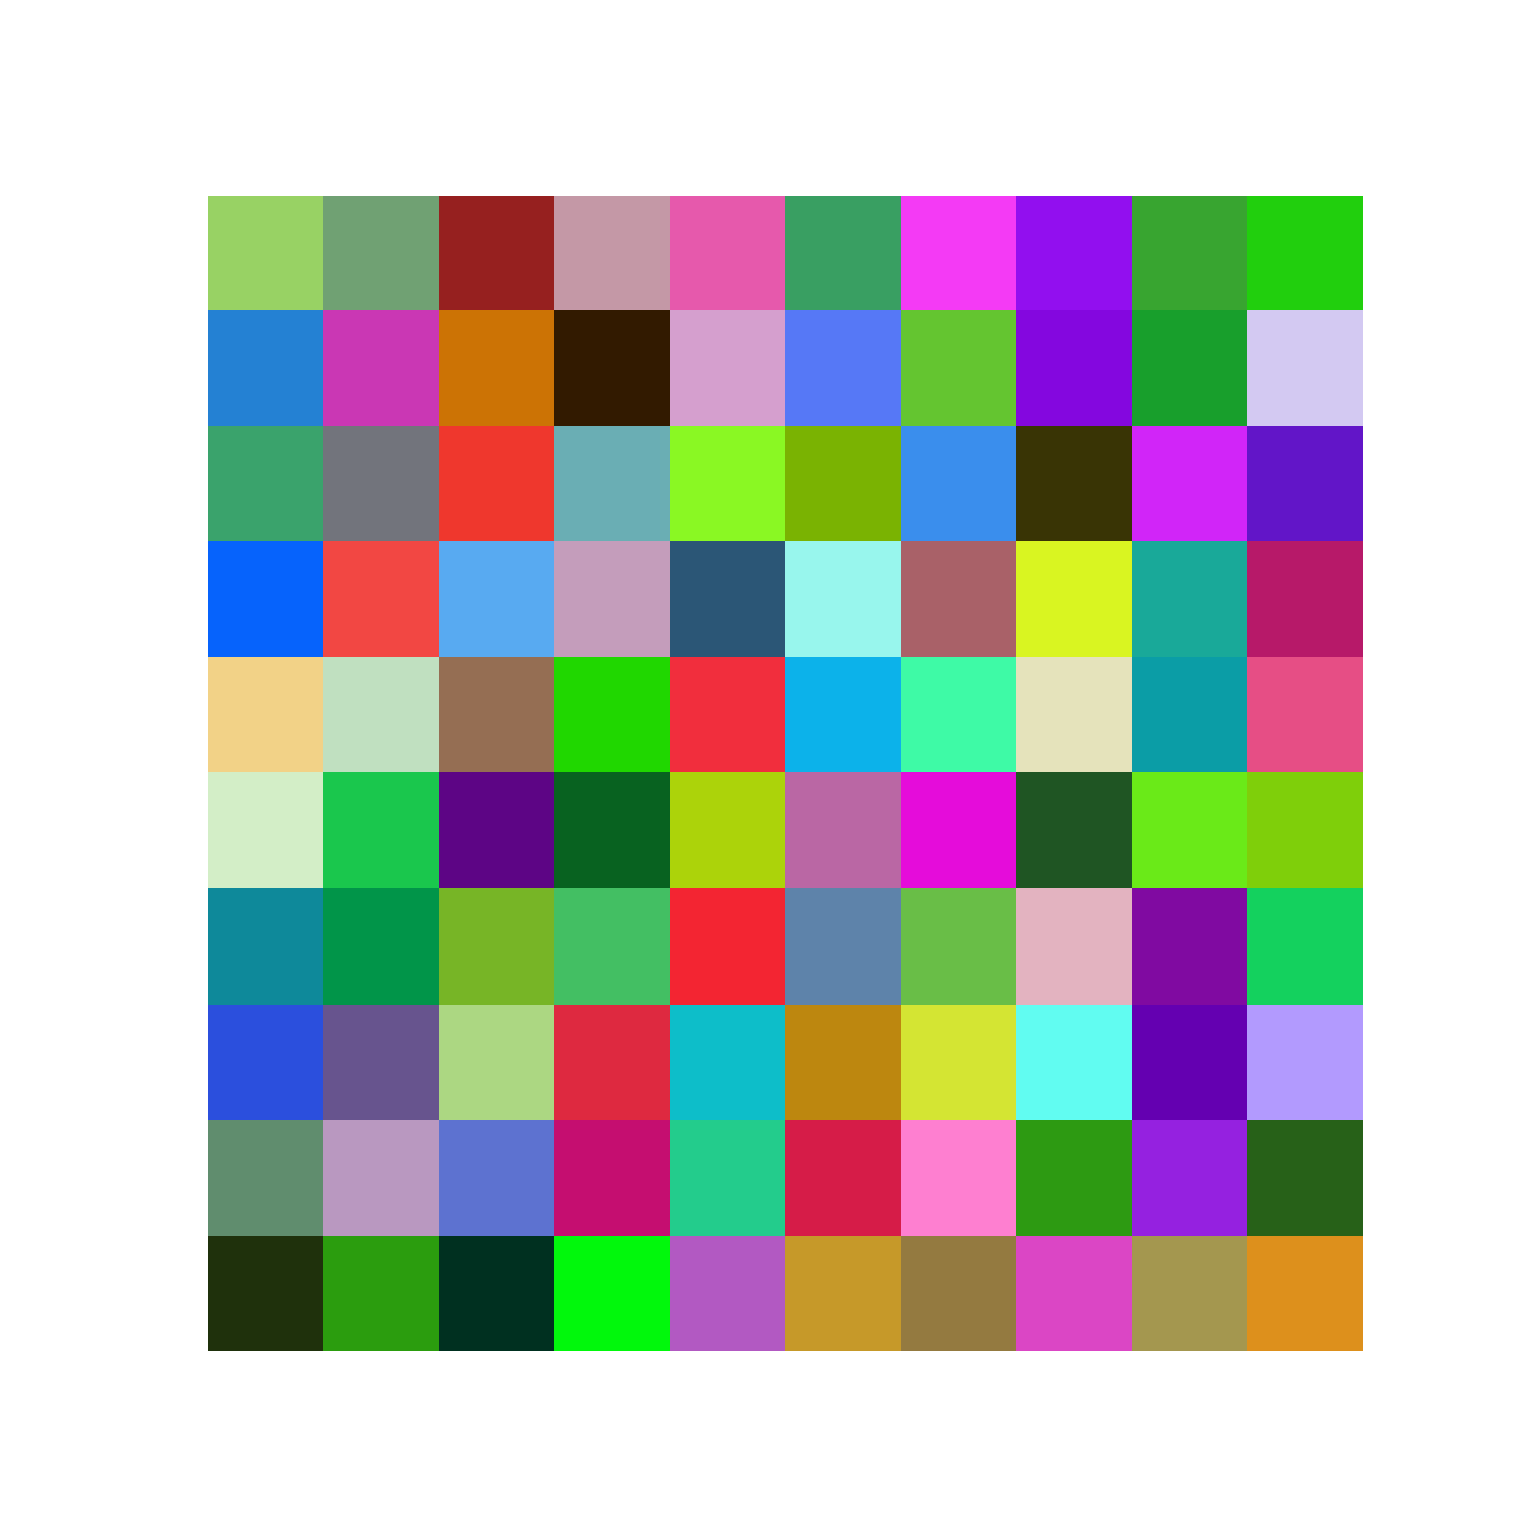
\includegraphics[width=.95\textwidth]{images/FE_img_rng_image.eps}
  \caption{Random image}
  \label{fig:channels}
\end{minipage}
\begin{minipage}[t]{.6\textwidth}
  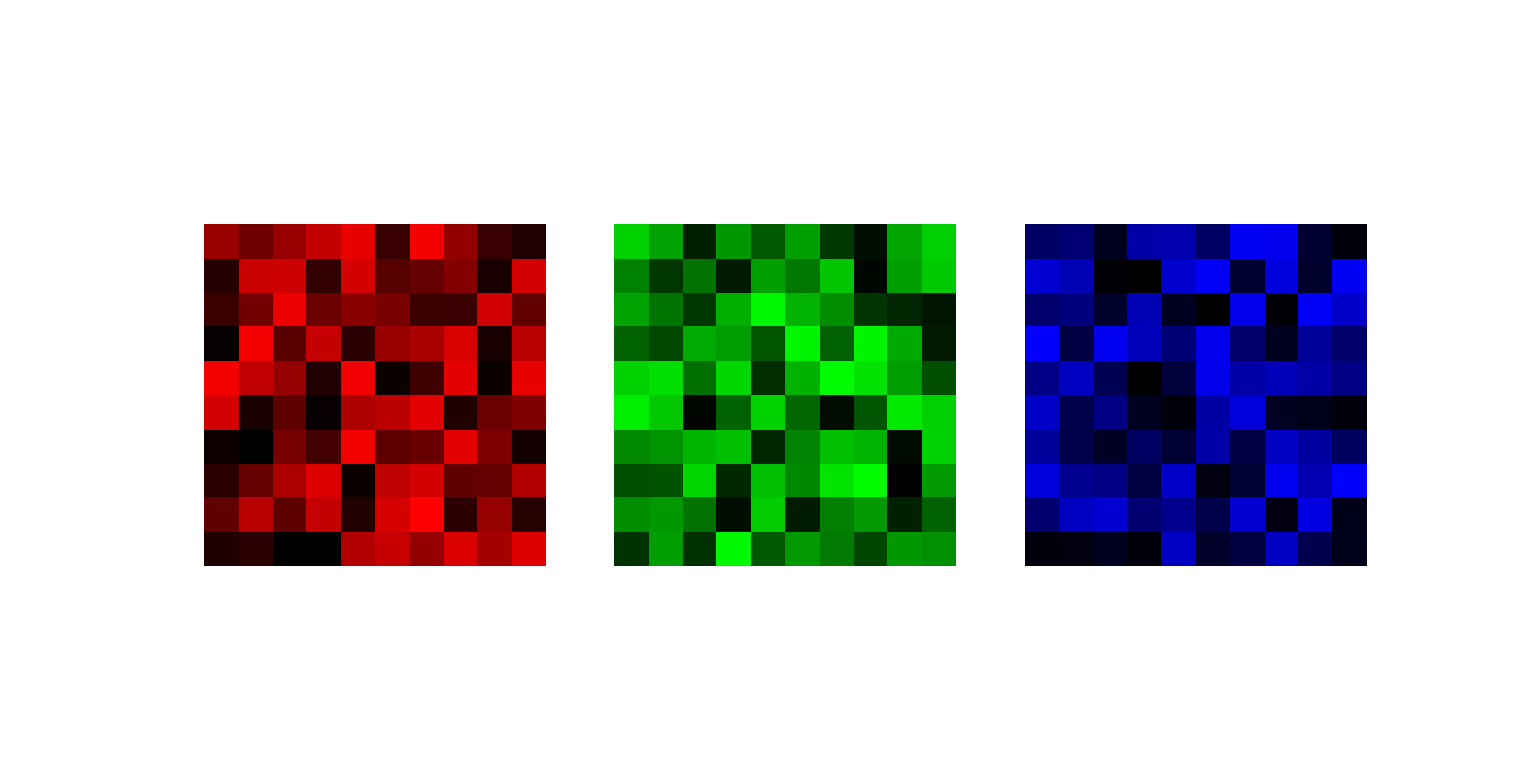
\includegraphics[width=.95\textwidth]{images/FE_img_channels.eps}
  \caption{Image channels individually}
  \label{fig:channels-individual}
\end{minipage}
\end{figure}

\framedtext{\color{red}{TODO:}} Implement example for CNN feature extraction

